\section{Tickets}
\label{sec:tickets}

The HOPR protocol makes use of a custom micropayment scheme to process its incentives. This section focuses on the utilized micro-payment scheme and serves as a building block for section \ref{sec:incentives}.

Incentives are handled by a structure called \textit{tickets} that is inspired by payment channels as well as probabilistic payments and allows nodes to issue asset transfers without requiring each time an on-chain interaction. Tickets are sent locked and get unlocked afterwards, i. e. after proving that a packet has been relayed. Nodes who receive a locked ticket are able to validate its validity. Once a node has received the required cryptographic material to unlock the ticket, it is able to claim the incentive by submitting the ticket to the smart contract.

\begin{figure}[H]
    \centering
    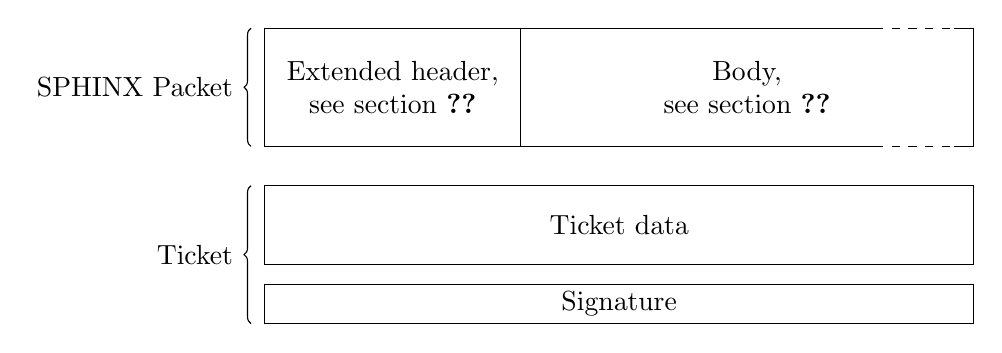
\begin{tikzpicture}[every text node part/.style={align=center}]
        \def\width{9}
        \def\headerWidth{9}
        \def\headerHeight{1.5}
        \def\headerOffset{3.25}
        \def\dashOffset{4.5}
        \def\dashWidth{1}

        \def\ticketDataHeight{1}
        \def\ticketSignatureHeight{0.5}

        \draw[decoration={brace,raise=5pt,mirror},decorate] (0,0) -- node[left=8pt] {SPHINX Packet} (0,-\headerHeight);

        \draw (0,0) rectangle (\headerOffset,-\headerHeight) node [midway] {Extended header,\\see section \ref{sec:incentives:proofofrelay}};
        \path [shape=rectangle] (\headerOffset,0) rectangle (\headerWidth,-\headerHeight) node [midway] {Body,\\see section \ref{sec:sphinx:payload}};

        \draw (\headerOffset+\dashOffset,-\headerHeight) -- (\headerOffset,-\headerHeight) -- (\headerOffset,0) -- (\headerOffset+\dashOffset,0);

        \draw [dashed] (\headerOffset+\dashOffset,0) -- (\headerOffset+\dashOffset+\dashWidth,0);
        \draw [dashed] (\headerOffset+\dashOffset,-\headerHeight) -- (\headerOffset+\dashOffset+\dashWidth,-\headerHeight);

        \draw (\headerOffset+\dashOffset+\dashWidth,-\headerHeight) -- (\headerWidth,-\headerHeight) -- (\headerWidth,0) -- (\headerOffset+\dashOffset+\dashWidth,0);

        \begin{scope}[shift={(0,-\headerHeight-0.5)}]
            \def\padding{0.25}

            \draw[decoration={brace,raise=5pt,mirror},decorate] (0,0) -- node[left=8pt] {Ticket} (0,-\ticketDataHeight-\padding-\ticketSignatureHeight);

            \draw (0,0) rectangle (\headerWidth,-\ticketDataHeight) node [midway] {Ticket data};

            \draw (0,-\ticketDataHeight-\padding) rectangle (\headerWidth,-\ticketDataHeight-\ticketSignatureHeight-\padding) node [midway] {Signature};
        \end{scope}
    \end{tikzpicture}
    \caption{Schematic overview of a mixnet packet that is sent together with a ticket.}
\end{figure}

\subimport{}{01-ticket-issuance.tex}
\subimport{}{02-ticket-validation.tex}
\subimport{}{03-ticket-redemption.tex}
